% ==========================================================================
% EscutAI · A Justiça que escuta você
% Pitch comercial · Hackathon TJPA · Desafio 3
% Compilar: pdflatex EscutAI_Pitch.tex (duas vezes, por causa das sobreposições TikZ)
% ==========================================================================
\documentclass[aspectratio=169,10pt]{beamer}

\usepackage[utf8]{inputenc}
\usepackage[T1]{fontenc}
\usepackage[brazil]{babel}
\usepackage[scaled=0.95]{helvet}
\renewcommand{\familydefault}{\sfdefault}
\usepackage{microtype}
\usepackage{graphicx}
\usepackage{booktabs}
\usepackage{tabularx}
\usepackage{array}
\usepackage{fontawesome5}
\usepackage{tikz}
\usetikzlibrary{arrows.meta,positioning,calc,shapes.geometric,fit,backgrounds,shadows}

% --------------------------------------------------------------------------
% Identidade visual (cores extraídas do pitch original)
% --------------------------------------------------------------------------
\definecolor{escuro}{HTML}{053F35}
\definecolor{petroleo}{HTML}{0B5345}
\definecolor{verde}{HTML}{00A884}
\definecolor{menta}{HTML}{16E0A9}
\definecolor{ambar}{HTML}{FDB833}
\definecolor{areia}{HTML}{FDE3A7}
\definecolor{nevoa}{HTML}{E8F4F0}
\definecolor{tinta}{HTML}{0E2F33}
\definecolor{cinza}{HTML}{5E6B6B}
\definecolor{seta}{HTML}{A8D5C6}

\setbeamercolor{normal text}{fg=tinta,bg=white}
\setbeamercolor{structure}{fg=petroleo}
\setbeamercolor{frametitle}{fg=tinta}
\setbeamercolor{itemize item}{fg=verde}
\setbeamercolor{itemize subitem}{fg=ambar}
\setbeamercolor{alerted text}{fg=verde}
\setbeamerfont{frametitle}{size=\LARGE,series=\bfseries}
\setbeamertemplate{navigation symbols}{}
\setbeamertemplate{itemize item}{\footnotesize\raise0.1ex\hbox{\textcolor{verde}{\faCaretRight}}}
\setbeamertemplate{itemize subitem}{\scriptsize\textcolor{ambar}{\faCircle}}
\setbeamersize{text margin left=0.75cm,text margin right=0.75cm}

\setbeamertemplate{frametitle}{%
  \vskip0.35cm
  \begin{minipage}[c]{0.70\paperwidth}\usebeamerfont{frametitle}\usebeamercolor[fg]{frametitle}\insertframetitle\end{minipage}%
  \hfill
  \begin{minipage}[c]{0.19\paperwidth}\raggedleft
    
\includegraphics[height=0.62cm]{img/logo_escutai_verde.png}\hspace{0.1cm}{\bfseries\small\textcolor{tinta}{Escut}\textcolor{verde}{AI}}%
  \end{minipage}\par
  \vskip-0.05cm
}

\setbeamertemplate{footline}{%
  \leavevmode\hbox to\paperwidth{%
    \hspace{0.75cm}{\tiny\textcolor{cinza}{EscutAI \textperiodcentered\ A Justiça que escuta você.}}\hfill
    {\tiny\textcolor{cinza}{\insertframenumber}}\hspace{0.75cm}}\vskip0.3cm}

% Slides escuros (capa, seções, encerramento)
\newcommand{\fundoescuro}{%
  \setbeamercolor{background canvas}{bg=escuro}%
  \setbeamercolor{normal text}{fg=white}%
  \setbeamertemplate{footline}{}%
  \setbeamertemplate{background}{%
    \begin{tikzpicture}[remember picture,overlay]
      \fill[petroleo,opacity=0.55] (current page.north west) circle (3.6cm);
      \fill[petroleo,opacity=0.40] (current page.south east) ++(-0.4,0.9) circle (4.1cm);
      \fill[petroleo,opacity=0.30] (current page.north east) circle (2.6cm);
    \end{tikzpicture}}%
  \usebeamercolor[fg]{normal text}}

% Imagem com reserva de espaço: se o arquivo ainda não existe, desenha um
% marcador com o nome esperado, para baixar depois (Pexels, Pixabay, Freepik)
\newcommand{\imagem}[4]{%
  \IfFileExists{#3}{\includegraphics[width=#1,height=#2,keepaspectratio]{#3}}{%
    \begin{tikzpicture}
      \node[draw=verde,dashed,rounded corners=6pt,fill=nevoa,minimum width=#1,minimum height=#2,
            align=center,font=\tiny,text=cinza,text width=#1-0.4cm]
           {\faImage\\[2pt]\texttt{\detokenize{#3}}\\[2pt]#4};
    \end{tikzpicture}}}

% Foto redonda para o slide do time
\newcommand{\fotoredonda}[2]{%
  \begin{tikzpicture}
    \begin{scope}
      \clip (0,0) circle (#2);
      \pgfmathsetlengthmacro{\diam}{2.05*#2}
      \node at (0,0) {\includegraphics[width=\diam]{#1}};
    \end{scope}
    \draw[menta,line width=1.4pt] (0,0) circle (#2);
  \end{tikzpicture}}

% Cartão de indicador
\newcommand{\kpi}[4]{%
  \begin{tikzpicture}
    \node[fill=nevoa,rounded corners=8pt,minimum width=4.35cm,minimum height=4.1cm] (c) {};
    \node[font=\fontsize{30}{32}\selectfont\bfseries,text=#4] at ($(c.center)+(0,0.85)$) {#1};
    \node[font=\normalsize\bfseries,text=#4,text width=3.9cm,align=center] at ($(c.center)+(0,-0.15)$) {#2};
    \node[font=\scriptsize,text=tinta,text width=3.9cm,align=center] at ($(c.center)+(0,-1.25)$)
         {\textcolor{ambar}{\faCircle}\ #3};
  \end{tikzpicture}}

% Estilos TikZ compartilhados
\tikzset{
  passo/.style={fill=petroleo,text=white,rounded corners=3pt,font=\tiny,align=center,
                text width=1.18cm,minimum height=0.66cm,inner sep=2pt},
  passoclaro/.style={passo,fill=verde},
  fim/.style={passo,fill=areia,text=ambar!60!black},
  canal/.style={rounded corners=5pt,text=white,font=\scriptsize\bfseries,align=left,
                minimum width=2.25cm,minimum height=0.74cm,inner sep=3pt},
  fluxo/.style={-{Triangle[width=5pt,length=4pt]},seta,line width=2.2pt},
  liga/.style={-{Stealth[length=5pt]},verde,line width=1pt},
  marco/.style={circle,fill=#1,minimum size=0.55cm,text=white,font=\scriptsize\bfseries},
  ciclo/.style={circle,fill=#1,text=white,minimum size=1.45cm,font=\tiny\bfseries,align=center,inner sep=1pt},
  caixa/.style={rounded corners=6pt,align=center,inner sep=4pt},
}

% Linha de etapas do diagrama de canais
\newcommand{\linha}[2]{%
  \foreach \t [count=\k from 0] in {#2}{
    \node[passo] (p#1-\k) at (4.35+1.5*\k,-#1) {\t};
  }}

% Fala da Julia com o ícone correspondente
\newcommand{\fala}[2]{\begin{minipage}[c]{1.15cm}\includegraphics[width=\linewidth]{img/julia_#1.png}\end{minipage}\hspace{4pt}%
  \begin{minipage}[c]{4.0cm}\scriptsize\itshape #2\end{minipage}\\[5pt]}

\title{EscutAI}
\subtitle{A Justiça que escuta você}
\author{Equipe EscutAI}
\date{Hackathon TJPA \textperiodcentered\ Desafio 3}

\begin{document}

% ==========================================================================
% 1. CAPA
% ==========================================================================
{\fundoescuro
\begin{frame}[plain]
  \begin{columns}[c]
    \column{0.55\textwidth}
      {\fontsize{34}{36}\selectfont\bfseries Pitch}\\[0.5cm]
      {\large\textcolor{menta!70!white}{Desafio 3 \textperiodcentered\ Melhoria do Atendimento\\Virtual e Presencial ao Jurisdicionado}}\\[0.9cm]
      {\small\textcolor{white!80}{\faWhatsapp\ WhatsApp oficial \quad\faInbox\ Chatwoot \quad\faRobot\ Assistente Julia}}
    \column{0.42\textwidth}
      \centering
      
\includegraphics[width=0.62\linewidth]{img/logo_escutai_branco.png}\\[0.25cm]
      {\fontsize{30}{32}\selectfont\bfseries Escut\textcolor{menta}{AI}}\\[0.15cm]
      {\small\textcolor{white!85}{A Justiça que escuta você.}}
  \end{columns}
\end{frame}
}

% ==========================================================================
% 2. TIME
% ==========================================================================
\begin{frame}{Nosso time}
  \centering
  \begin{tikzpicture}[pessoa/.style={align=center,font=\footnotesize}]
    \foreach \x/\arq/\nome/\papel in {
      0/carlos_portela/Carlos Portela/Gestão de Negócios,
      4.4/elton_sarmanho/Elton Sarmanho/TI e Comunicação,
      8.8/eduardo_chaves/Eduardo Chaves/Conhecimento de Negócio}{
      \node at (\x,0) {\fotoredonda{img/time_\arq.png}{0.82cm}};
      \node[pessoa] at (\x,-1.3) {\textbf{\nome}\\\textcolor{verde}{\papel}};
    }
    \foreach \x/\arq/\nome/\papel in {
      2.2/marcio_furtado/Márcio Furtado/Design,
      6.6/josue_ferreira/Josué Ferreira/Experiência do Usuário}{
      \node at (\x,-2.95) {\fotoredonda{img/time_\arq.png}{0.82cm}};
      \node[pessoa] at (\x,-4.25) {\textbf{\nome}\\\textcolor{verde}{\papel}};
    }
  \end{tikzpicture}
  \vfill
  {\small Negócio, direito, tecnologia e design na mesma mesa. Por isso o protótipo saiu do papel e já roda no WhatsApp.}
\end{frame}

% ==========================================================================
% 3. O TAMANHO DO PROBLEMA
% ==========================================================================
\begin{frame}{A sobrecarga do atendimento}
  \centering
  \kpi{1.747.124}{solicitações de atendimento}{Média de ago.\ e set.\ (60 dias)}{verde}\hfill
  \kpi{55\%}{atendimentos realizados}{962.259 atendidos, ou seja, 784.865 pedidos ficaram sem resposta}{petroleo}\hfill
  \kpi{3.218}{atendimentos por unidade}{5.843 solicitações por unidade}{verde}
  \vfill
  \begin{tikzpicture}
    \node[fill=areia,rounded corners=4pt,text width=13.9cm,inner sep=6pt,font=\small,text=ambar!45!black]
      {\faExclamationCircle\ Quase metade das pessoas que procuram o Tribunal não é atendida no período. E o país fechou 2024 com 80,6 milhões de processos pendentes e 39,4 milhões de casos novos \cite{cnj2025}, então a demanda por informação processual não vai cair sozinha.};
  \end{tikzpicture}\\[2pt]
  {\tiny\textcolor{cinza}{Indicadores do TJPA levantados pela equipe (média de agosto e setembro). Diferença entre solicitações e atendimentos calculada a partir desses números.}}
\end{frame}

% ==========================================================================
% 4. CANAIS FRAGMENTADOS (diagrama redesenhado em TikZ)
% ==========================================================================
\begin{frame}{Cinco portas que não conversam}
  \centering
  \resizebox{\linewidth}{!}{%
  \begin{tikzpicture}[x=1cm,y=1cm]
    \node[fill=verde,text=white,rounded corners=6pt,minimum width=1.7cm,minimum height=2.3cm,
          align=center,font=\scriptsize\bfseries] (u) at (-0.2,-2) {\Large\faUser\\[3pt]Usuário\\precisa de\\atendimento};
    % canal, cor, ícone, etapas
    \foreach \i/\nome/\icone/\cor in {
        0/{Presencial na\\Secretaria}/\faUniversity/escuro,
        1/{Balcão\\Virtual}/\faDesktop/verde,
        2/{WhatsApp\\(não oficial)}/\faWhatsapp/escuro,
        3/{Telefone}/\faPhone/verde,
        4/{E-mail}/\faEnvelope/escuro}{
      \node[canal,fill=\cor] (c\i) at (2.35,-\i) {\makebox[0.55cm][l]{\large\icone}\parbox{1.45cm}{\nome}};
      \draw[-{Stealth[length=5pt]},escuro,line width=1.1pt] (u.east) to[out=0,in=180] (c\i.west);
    }
    \linha{0}{Desloca-se à unidade,Informa o nº do processo,Servidor consulta sistemas}
    \linha{1}{Acessa site e sistema,Solicita atendimento,Aguarda fila virtual,Entra na sala virtual,Informa dados,Servidor consulta sistemas}
    \linha{2}{Localiza canal local,Contato direto com servidor,Servidor consulta e responde}
    \linha{3}{Consulta lista no site,Liga para a unidade,Atendente consulta e informa}
    \linha{4}{Consulta lista no site,Envia solicitação,Servidor verifica e-mail,Consulta e responde}
    \foreach \i/\n in {0/3,1/6,2/3,3/3,4/4}{
      \node[fim] (f\i) at (4.35+1.5*\n,-\i) {Recebe a informação};
      \draw[fluxo] (c\i.east) -- (p\i-0.west);
      \pgfmathtruncatemacro{\ult}{\n-1}
      \foreach \k in {1,...,\ult}{
        \pgfmathtruncatemacro{\ant}{\k-1}
        \draw[fluxo] (p\i-\ant.east) -- (p\i-\k.west);
      }
      \draw[fluxo] (p\i-\ult.east) -- (f\i.west);
    }
  \end{tikzpicture}}
  \vspace{0.15cm}

  \begin{tikzpicture}
    \node[fill=areia,rounded corners=4pt,text width=13.9cm,inner sep=5pt,font=\small,text=ambar!45!black]
      {\faExclamationTriangle\ Todo caminho termina no mesmo ponto: um servidor consultando o sistema para repassar uma informação básica (andamento, fluxo, orientação simples) que não exigiria atendimento humano.};
  \end{tikzpicture}
\end{frame}

% ==========================================================================
% 5. CUSTO DA FRAGMENTAÇÃO (tabela booktabs)
% ==========================================================================
\begin{frame}{O que a fragmentação custa}
  \footnotesize
  \begin{tabularx}{\linewidth}{@{}l c c X@{}}
    \toprule
    \textbf{Canal} & \textbf{Etapas até a resposta} & \textbf{Depende de servidor} & \textbf{Onde fica o histórico} \\
    \midrule
    \faUniversity\ Presencial    & 4 & sim & na memória de quem atendeu \\
    \faDesktop\ Balcão Virtual   & 7 & sim & sala de vídeo, sem registro da conversa \\
    \faWhatsapp\ WhatsApp local  & 4 & sim & celular da unidade, fora de qualquer sistema \\
    \faPhone\ Telefone           & 4 & sim & não fica registrado \\
    \faEnvelope\ E-mail          & 5 & sim & caixa de cada unidade \\
    \midrule
    \textbf{EscutAI}             & \textbf{2} & \textbf{só quando precisa} & \textbf{uma caixa única, com ticket, data e hora} \\
    \bottomrule
  \end{tabularx}
  \vspace{0.15cm}

  \begin{columns}[T]
    \column{0.5\textwidth}
      \textbf{\textcolor{petroleo}{\faUser\ Para o cidadão}}
      \begin{itemize}\footnotesize
        \item precisa descobrir qual canal funciona na sua unidade
        \item repete os mesmos dados a cada contato
      \end{itemize}
    \column{0.5\textwidth}
      \textbf{\textcolor{petroleo}{\faUserTie\ Para o Tribunal}}
      \begin{itemize}\footnotesize
        \item ninguém enxerga a fila completa nem mede o tempo de resposta
        \item servidores gastam o dia em perguntas repetidas
      \end{itemize}
  \end{columns}
  \vfill
  {\tiny\textcolor{cinza}{Contagem de etapas a partir do mapeamento de jornadas da equipe (slide anterior). Coluna de histórico: diagnóstico qualitativo da equipe.}}
\end{frame}

% ==========================================================================
% 6. QUEM SOFRE
% ==========================================================================
\begin{frame}{Quem sofre com isso}
  \centering
  \begin{columns}[T]
    \column{0.49\textwidth}\centering
      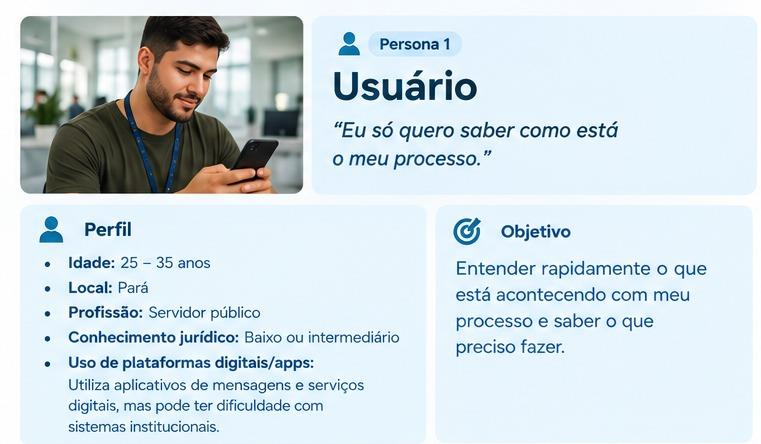
\includegraphics[width=\linewidth]{img/persona_usuario_card.png}\\[4pt]
      \begin{tikzpicture}
        \node[fill=nevoa,rounded corners=5pt,text width=0.92\linewidth,inner sep=6pt,font=\small]
          {\textbf{\textcolor{petroleo}{Objetivo:}} entender rápido o que está acontecendo com o processo e saber o que fazer. Usa WhatsApp todo dia, mas se perde nos sistemas do Tribunal.};
      \end{tikzpicture}
    \column{0.49\textwidth}\centering
      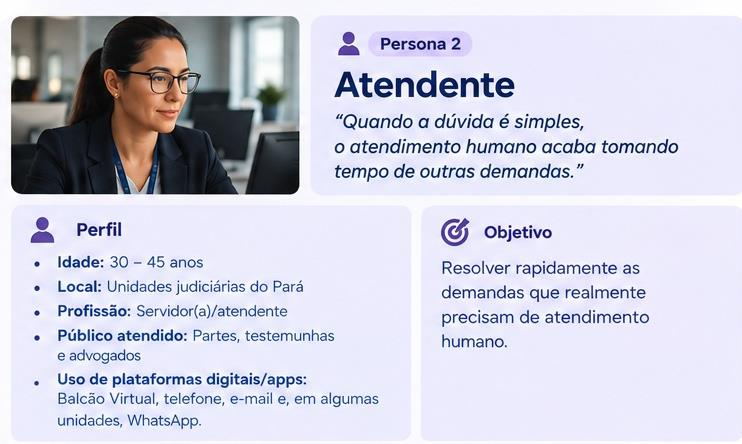
\includegraphics[width=\linewidth]{img/persona_atendente_card.png}\\[4pt]
      \begin{tikzpicture}
        \node[fill=nevoa,rounded corners=5pt,text width=0.92\linewidth,inner sep=6pt,font=\small]
          {\textbf{\textcolor{petroleo}{Objetivo:}} dedicar seu tempo às demandas que realmente pedem análise humana, e não ao décimo pedido de andamento do dia.};
      \end{tikzpicture}
  \end{columns}
\end{frame}

% ==========================================================================
% 7. SEÇÃO: NOSSA SOLUÇÃO
% ==========================================================================
{\fundoescuro
\begin{frame}[plain]
  \begin{columns}[c]
    \column{0.55\textwidth}
      {\fontsize{32}{34}\selectfont\bfseries Nossa solução}\\[0.4cm]
      {\large\textcolor{menta!70!white}{Uma porta de entrada oficial, uma central que organiza tudo e uma assistente que responde com fonte.}}
    \column{0.40\textwidth}\centering
      
\includegraphics[width=0.85\linewidth]{img/julia_oi.png}
  \end{columns}
\end{frame}
}

% ==========================================================================
% 8. VISÃO: TODOS OS CANAIS EM UMA CENTRAL
% ==========================================================================
\begin{frame}{Todos os canais chegam ao mesmo lugar}
  \centering
  \definecolor{arqCanal}{HTML}{EAF1F3}
  \definecolor{arqCanalB}{HTML}{0E4F5C}
  \definecolor{arqOrq}{HTML}{E5484D}
  \definecolor{arqOrqF}{HTML}{FDECEC}
  \definecolor{arqHub}{HTML}{1F2A33}
  \definecolor{arqDB}{HTML}{F2A93B}
  \definecolor{arqDBF}{HTML}{FDF3E1}
  \definecolor{arqIA}{HTML}{7A1F5C}
  \definecolor{arqIAF}{HTML}{F6ECF3}
  \definecolor{arqHum}{HTML}{F2B33D}
  \definecolor{arqHumF}{HTML}{FDEFC4}
  \definecolor{arqSeta}{HTML}{5B6573}
  \resizebox{!}{6.1cm}{%
  \begin{tikzpicture}[x=1cm,y=1cm,font=\sffamily,
      box/.style={rounded corners=3pt,align=center,line width=0.9pt,inner sep=4pt},
      canalA/.style={box,fill=arqCanal,draw=arqCanalB,text width=2.9cm,minimum height=1.05cm},
      sub/.style={box,fill=white,draw=arqOrq,text width=3.0cm,minimum height=0.95cm},
      seta/.style={-{Stealth[length=6pt,width=5pt]},arqSeta,line width=0.9pt},
      seta2/.style={{Stealth[length=6pt,width=5pt]}-{Stealth[length=6pt,width=5pt]},arqSeta,line width=0.9pt},
      rot/.style={font=\footnotesize,text=arqSeta,align=center,fill=white,inner sep=1.5pt}]

    % Canais de entrada
    \node[canalA] (wa) at (0,1.1)  {\faWhatsapp\ \textbf{WhatsApp}\\{\footnotesize (Meta Cloud API)}};
    \node[canalA] (em) at (0,-1.1) {\faEnvelope\ \textbf{E-mail}\\{\footnotesize (inbox de e-mail)}};
    \node[draw=gray!50,dashed,rounded corners=6pt,fit=(wa)(em),inner sep=8pt] (gcan) {};
    \node[font=\footnotesize,text=gray!80!black,above=1pt of gcan] {Canais de entrada};

    % Orquestrador
    \node[box,fill=arqOrqF,draw=arqOrq,line width=1.2pt,text width=4.5cm,minimum height=1.15cm] (core) at (7.4,0)
      {\faMicrochip\ \textbf{EscutAI Orquestrador}\\\textbf{\footnotesize FastAPI + Agno}};
    \node[sub] (tk) at (5.6,2.7) {\faListOl\ \textbf{Ticket Flow}\\{\footnotesize TKT e máquina de estados}};
    \node[sub] (rt) at (9.3,2.7) {\faRoute\ \textbf{Roteamento}\\{\footnotesize menus, times e transbordo}};
    \begin{pgfonlayer}{background}
      \node[draw=arqOrq!55,dashed,rounded corners=8pt,fit=(tk)(rt)(core),inner xsep=14pt,inner ysep=10pt] (gorq) {};
    \end{pgfonlayer}
    \node[font=\footnotesize,text=arqOrq,above=1pt of gorq] {Orquestrador};
    \draw[seta] (tk.south |- core.north) -- (tk.south);
    \draw[seta] (rt.south |- core.north) -- (rt.south);

    % Webhooks das inboxes (rótulo no meio, setas para o canal e para o orquestrador)
    \foreach \c/\y/\t in {wa/0.85/{webhook da inbox\\WhatsApp},em/-0.85/{webhook da inbox\\E-mail}}{
      \node[rot] (r\c) at (3.55,\y) {\t};
      \draw[seta] (r\c.west) -- (\c.east);
      \draw[seta] (r\c.east) -- (core.west);
    }

    % Chatwoot
    \node[box,fill=arqHub,draw=arqHub,text=white,text width=3.3cm,minimum height=1.15cm] (cw) at (15.0,0)
      {\faComments\ \textbf{Chatwoot}\\\textbf{\footnotesize Hub de Atendimento}};
    \draw[seta] (core.east) -- (cw.west);
    \node[rot,anchor=south] at (11.6,0.12) {API de agente:\\mensagens, \textit{labels},\\time, botões};

    % Atendente humano
    \node[box,fill=arqHumF,draw=arqHum,text width=3.3cm,minimum height=1.05cm] (hum) at (15.0,-3.1)
      {\faHeadset\ \textbf{Atendente humano}\\{\footnotesize interface do Chatwoot}};
    \draw[seta] (cw.south) -- (hum.north);
    \node[rot,anchor=west] at (15.1,-1.55) {transbordo\\e histórico};

    % Julia (IA)
    \node[box,fill=arqIAF,draw=arqIA,text width=3.3cm,minimum height=1.05cm] (ia) at (5.6,-3.1)
      {\faRobot\ \textbf{Julia}\\{\footnotesize IA RAG (MariTalk Sabiá)}};
    \draw[seta2] (ia.north) -- (ia.north |- core.south);

    % Base de conhecimento
    \node[cylinder,shape border rotate=90,aspect=0.22,draw=arqDB,fill=arqDBF,line width=1pt,
          minimum width=3.6cm,minimum height=1.9cm,align=center] (db) at (9.4,-3.3)
      {\faDatabase\ \textbf{Base curada}\\{\footnotesize SQLite: BM25 + vetores}\\{\footnotesize tickets e auditoria}};
    \draw[seta2] (db.north |- core.south) -- (db.north);
  \end{tikzpicture}}
  \vfill
  {\tiny\textcolor{cinza}{Balcão Virtual e consulta processual são opções do menu dentro da conversa no WhatsApp.}}
\end{frame}

% ==========================================================================
% 9. COMO RESOLVEREMOS (três jornadas)
% ==========================================================================
\begin{frame}{Como resolvemos cada tipo de demanda}
  \centering
  \begin{tikzpicture}[x=1cm,y=1cm,
      etapa/.style={caixa,fill=verde,text=white,font=\scriptsize,minimum width=1.95cm,minimum height=0.85cm,text width=1.8cm},
      etapaf/.style={etapa,fill=areia,text=ambar!45!black},
      num/.style={circle,fill=menta,text=escuro,font=\scriptsize\bfseries,inner sep=1.2pt,minimum size=0.42cm},
      numf/.style={num,fill=ambar,text=white},
      rot/.style={font=\small\bfseries,text=tinta,anchor=west}]
    % Dúvidas frequentes
    \node[rot] at (-0.95,3.2) {\textcolor{ambar}{\faCircle}\ Dúvidas frequentes};
    \node[etapa] (a1) at (0,2.4) {\faWhatsapp\\Início do atendimento};
    \node[etapaf] (a2) at (2.45,2.4) {\faRobot\\Julia responde};
    \node[num] at (a1.north west) {1}; \node[numf] at (a2.north west) {2};
    \draw[fluxo] (a1) -- (a2);
    % Perguntas sobre processos
    \node[rot] at (-0.95,1.1) {\textcolor{ambar}{\faCircle}\ Perguntas sobre processos};
    \foreach \t/\ic [count=\k] in {Início do atendimento/\faWhatsapp,Julia identifica o processo/\faRobot,Leitura dos documentos/\faFolderOpen}{
      \node[etapa] (b\k) at (2.45*\k-2.45,0.2) {\ic\\\t};
      \node[num] at (b\k.north west) {\k};
    }
    \node[etapaf] (b4) at (7.35,0.2) {\faComments\\Perguntas e respostas};
    \node[numf] at (b4.north west) {4};
    \foreach \k [evaluate=\k as \j using int(\k+1)] in {1,2,3}{\draw[fluxo] (b\k) -- (b\j);}
    % Casos complexos
    \node[rot] at (-0.95,-0.9) {\textcolor{ambar}{\faCircle}\ Casos mais complexos};
    \foreach \t/\ic [count=\k] in {Início do atendimento/\faWhatsapp,Julia identifica o processo/\faRobot,Leitura dos documentos/\faFolderOpen,Perguntas e respostas/\faComments,Atendimento humano/\faUserTie}{
      \node[etapa] (c\k) at (2.45*\k-2.45,-2.0) {\ic\\\t};
      \node[num] at (c\k.north west) {\k};
    }
    \node[etapaf] (c6) at (12.25,-2.0) {\faIcon{ticket-alt}\\Ticket e acompanhamento};
    \node[numf] at (c6.north west) {6};
    \foreach \k [evaluate=\k as \j using int(\k+1)] in {1,...,5}{\draw[fluxo] (c\k) -- (c\j);}
  \end{tikzpicture}
  \vfill
  {\small A pessoa sai da conversa sabendo a resposta ou sabendo quem vai responder. Nunca fica sem retorno.}
\end{frame}

% ==========================================================================
% 10. JULIA
% ==========================================================================
\begin{frame}{Julia, a ouvidora acolhedora}
  \begin{columns}[c]
    \column{0.27\textwidth}\centering
      
\includegraphics[width=0.95\linewidth]{img/julia_mascote.png}\\
      {\Large\bfseries\textcolor{verde}{JULIA}}
    \column{0.33\textwidth}
      \begin{tikzpicture}
        \node[fill=nevoa,rounded corners=8pt,text width=4.4cm,inner sep=8pt,font=\small] (t) {%
          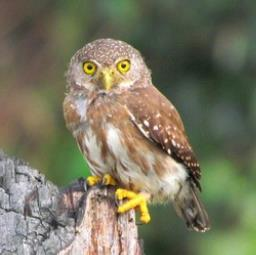
\includegraphics[width=1.0cm]{img/julia_cabure.png}\hspace{4pt}\textbf{\textcolor{ambar!70!black}{Caburé-da-amazônia}}\\[6pt]
          \textcolor{verde}{\faCheck}\ A coruja une conhecimento jurídico e escuta atenta. Corujas estão entre os animais de audição mais sensível.\\[4pt]
          \textcolor{verde}{\faCheck}\ Quem chega com dúvida encontra alguém que ouve primeiro e explica depois.\\[4pt]
          \textcolor{verde}{\faCheck}\ O fone de ouvido lembra o compromisso: escutar antes de responder.};
      \end{tikzpicture}
    \column{0.38\textwidth}
      \fala{oi}{``Oi! Eu sou a Julia. Estou aqui para te ouvir. Como posso te ajudar hoje?''}
      \fala{verificando}{``Se entendi bem, você quer saber como está o seu processo. Vou verificar agora.''}
      \fala{encaminhando}{``Essa parte precisa de um atendimento humano. Vou te encaminhar para a equipe do Balcão Virtual.''}
      \fala{duvida}{``Essa dúvida eu não consigo responder com segurança. Vou encaminhar para quem pode responder.''}
  \end{columns}
\end{frame}

% ==========================================================================
% 11. ARQUITETURA MACRO
% ==========================================================================
\begin{frame}{Arquitetura em visão macro}
  \centering
  \begin{tikzpicture}[x=1cm,y=1cm,
      camada/.style={rounded corners=6pt,minimum width=10.6cm,minimum height=1.0cm},
      rotulo/.style={anchor=west,font=\small\bfseries,text width=2.6cm},
      desc/.style={anchor=west,font=\scriptsize,text width=7.6cm},
      chip/.style={fill=white,text=petroleo,font=\tiny\bfseries,inner sep=3pt,rounded corners=3pt,anchor=west}]
    \foreach \y/\cor/\txt/\rot/\d in {
        3.0/nevoa/petroleo/{\faComments\ 1. Canais}/{},
        1.75/verde/white/{\faInbox\ 2. Central}/{Fila única, times por assunto, etiquetas, transferência para humano e tickets com data e hora},
        0.5/petroleo/white/{\faRobot\ 3. Inteligência}/{A Julia entende o pedido, busca a evidência, responde com fonte e confere antes de enviar},
        -0.75/escuro/white/{\faBook\ 4. Conhecimento}/{Processos, informação institucional e orientação jurídica, sempre com conteúdo aprovado}}{
      \node[camada,fill=\cor] (L) at (0,\y) {};
      \node[rotulo,text=\txt] at ($(L.west)+(0.15,0)$) {\rot};
      \node[desc,text=\txt] at ($(L.west)+(2.85,0)$) {\d};
    }
    \node[chip,fill=verde,text=white] at (-2.0,3.0) {\faWhatsapp\ WhatsApp oficial};
    \node[chip] at (0.4,3.0) {\faEnvelope\ E-mail};
    \foreach \y in {2.375,1.125,-0.125}{
      \draw[{Stealth[length=4pt]}-{Stealth[length=4pt]},ambar,line width=1.3pt] (4.75,\y+0.13) -- (4.75,\y-0.13);}
    \node[rounded corners=6pt,fill=areia,minimum height=4.75cm,text width=2.5cm,font=\scriptsize,align=center,anchor=north west,inner sep=5pt]
      at (5.6,3.5)
      {\textbf{\faIcon{shield-alt}\ Governança}\\[6pt]
       curadoria humana do conteúdo\\[5pt]
       dados pessoais mascarados (LGPD)\\[5pt]
       registro de auditoria\\[5pt]
       supervisão humana (CNJ 615/2025)};
    \node[rounded corners=6pt,draw=verde,dashed,minimum width=10.6cm,text width=10.2cm,font=\scriptsize,align=center,inner sep=5pt]
      at (0,-1.85)
      {\faPlug\ \textbf{Integrações previstas:} API processual oficial (PJe), agenda do Balcão Virtual no menu do WhatsApp, indicadores no painel do Tribunal};
  \end{tikzpicture}
\end{frame}

% ==========================================================================
% 12. RESPOSTA SEGURA
% ==========================================================================
\begin{frame}{Como a Julia evita inventar respostas}
  \centering
  \begin{tikzpicture}[x=1cm,y=1cm,
      etapa/.style={caixa,fill=nevoa,font=\scriptsize,minimum height=1.55cm,text width=2.05cm,minimum width=2.25cm},
      forte/.style={etapa,fill=verde,text=white}]
    \node[etapa] (e1) at (0,0)    {{\Large\textcolor{verde}{\faComment}}\\[2pt]\textbf{Pergunta}\\em linguagem do dia a dia};
    \node[etapa] (e2) at (2.75,0) {{\Large\textcolor{verde}{\faSearch}}\\[2pt]\textbf{Entende}\\assunto e processo da conversa};
    \node[etapa] (e3) at (5.5,0)  {{\Large\textcolor{verde}{\faFolderOpen}}\\[2pt]\textbf{Busca}\\só em documentos aprovados};
    \node[etapa] (e4) at (8.25,0) {{\Large\textcolor{verde}{\faPenNib}}\\[2pt]\textbf{Escreve}\\citando o trecho usado};
    \node[forte] (e5) at (11.0,0) {{\Large\faClipboardCheck}\\[2pt]\textbf{Confere}\\datas, valores e números contra a fonte};
    \foreach \a/\b in {e1/e2,e2/e3,e3/e4,e4/e5}{\draw[fluxo] (\a) -- (\b);}
    \node[caixa,fill=petroleo,text=white,font=\scriptsize,text width=4.4cm,minimum height=1.0cm] (ok) at (10.0,-2.25)
      {\faCheckCircle\ \textbf{Confirmou:} responde em linguagem simples, com a fonte};
    \node[caixa,fill=areia,text=ambar!40!black,font=\scriptsize,text width=4.4cm,minimum height=1.0cm] (nao) at (4.0,-2.25)
      {\faHandPaper\ \textbf{Não achou evidência:} diz que não sabe e oferece um atendente};
    \draw[liga] (e5.south) -- ++(0,-0.45) -| (ok.north);
    \draw[liga] (e5.south) -- ++(0,-0.45) -| (nao.north);
  \end{tikzpicture}
  \vfill
  \begin{tikzpicture}
    \node[fill=nevoa,rounded corners=4pt,text width=13.9cm,inner sep=6pt,font=\small]
      {Essa técnica se chama \textbf{geração aumentada por recuperação} (RAG). A literatura mostra que ela torna as respostas mais factuais \cite{lewis2020} e reduz alucinações em mais de 60\% \cite{shuster2021}. Ferramentas jurídicas comerciais ainda erram entre 17\% e 33\% das vezes \cite{magesh2025}, por isso a Julia confere cada resposta e prefere se calar a chutar.};
  \end{tikzpicture}
\end{frame}

% ==========================================================================
% 12b. ABORDAGEM TÉCNICA
% ==========================================================================
\begin{frame}{Abordagem técnica: RAG híbrido}
  \centering
  \begin{tikzpicture}[x=1cm,y=1cm,
      bloco/.style={caixa,fill=nevoa,font=\scriptsize,text width=2.1cm,minimum height=1.05cm},
      escuro/.style={bloco,fill=petroleo,text=white},
      filtro/.style={caixa,fill=areia,font=\scriptsize,text width=2.1cm,minimum height=1.05cm,text=ambar!40!black}]
    \node[bloco] (q) at (0,0) {\faComment\ \textbf{Pergunta}\\+ processo em foco na conversa};
    \node[bloco] (l) at (2.75,0.68) {\textbf{Busca lexical}\\BM25 com radicais do português};
    \node[bloco] (v) at (2.75,-0.68) {\textbf{Busca semântica}\\vetores multilíngues};
    \node[escuro] (r) at (5.5,0) {\textbf{Fusão RRF}\\une os dois rankings};
    \node[filtro] (f) at (8.25,0) {\textbf{Filtros}\\só aprovado, processo, data, tipo de peça};
    \node[escuro] (g) at (11.0,0) {\textbf{LLM brasileiro}\\escreve com citação [n]};
    \node[bloco,fill=verde,text=white] (c) at (11.0,-2.0) {\faClipboardCheck\ \textbf{Verificador}\\datas, valores, artigos, números};
    \node[bloco] (a) at (5.5,-2.0) {\faHandPaper\ \textbf{Abstenção}\\pouca evidência ou fonte não confere};
    \node[bloco,fill=areia] (ok) at (8.25,-2.0) {\faCheckCircle\ \textbf{Resposta}\\com fonte e página};
    \draw[liga] (q.east) -- (l.west); \draw[liga] (q.east) -- (v.west);
    \draw[liga] (l.east) -- (r.west); \draw[liga] (v.east) -- (r.west);
    \draw[fluxo] (r) -- (f); \draw[fluxo] (f) -- (g); \draw[fluxo] (g) -- (c);
    \draw[fluxo] (c) -- (ok);
    \draw[liga,dashed] (c.south) -- ++(0,-0.35) -| (a.south);
  \end{tikzpicture}
  \vspace{0.1cm}

  \scriptsize
  \begin{tabularx}{\linewidth}{@{}l X l X@{}}
    \toprule
    \textbf{Camada} & \textbf{Tecnologia} & \textbf{Camada} & \textbf{Tecnologia} \\
    \midrule
    Canal e central   & WhatsApp Cloud API, Chatwoot (MIT) & Busca      & SQLite FTS5 (BM25), embeddings MiniLM multilíngue, RRF \\
    Serviço           & Python, FastAPI, Agno (agente)      & Geração    & MariTalk Sabiá, modelo treinado em português \\
    Leitura de PDF    & pdftotext, OCR Tesseract, leitor de capa do PJe & Implantação & Docker na VM, atrás do mesmo Nginx do Chatwoot \\
    \bottomrule
  \end{tabularx}
\end{frame}

% ==========================================================================
% 12c. METODOLOGIA
% ==========================================================================
\begin{frame}{Metodologia de trabalho}
  \begin{columns}[c]
    \column{0.47\textwidth}\centering
    \begin{tikzpicture}[x=1cm,y=1cm]
      \foreach \ang/\cor/\txt [count=\k] in {
          90/verde/{1\\Diagnóstico},
          30/petroleo/{2\\Especificação},
          -30/verde/{3\\Curadoria},
          -90/petroleo/{4\\Construção},
          -150/verde/{5\\Avaliação},
          150/ambar/{6\\Validação}}{
        \node[ciclo=\cor] (n\k) at (\ang:2.05) {\txt};
      }
      \foreach \a/\b in {1/2,2/3,3/4,4/5,5/6,6/1}{
        \draw[-{Stealth[length=5pt]},seta,line width=1.6pt] (n\a) to[bend left=18] (n\b);}
      \node[font=\scriptsize\bfseries,text=petroleo,align=center] at (0,0) {ciclo curto\\e medido};
    \end{tikzpicture}
    \column{0.51\textwidth}
    \scriptsize
    \begin{enumerate}\setlength\itemsep{2pt}
      \item[\textbf{1}] \textbf{Diagnóstico} do problema e do acervo, separando o que é confirmado, inferido e desconhecido.
      \item[\textbf{2}] \textbf{Especificação} com requisitos testáveis e 17 situações de atendimento a cobrir.
      \item[\textbf{3}] \textbf{Curadoria}: triagem automática (segredo de justiça, dados pessoais) e aprovação humana.
      \item[\textbf{4}] \textbf{Construção incremental} em arquitetura limpa (domínio, aplicação, infraestrutura), com testes a cada passo.
      \item[\textbf{5}] \textbf{Avaliação} com perguntas e respostas de referência, separando o conjunto de ajuste dos conjuntos de validação.
      \item[\textbf{6}] \textbf{Validação} por revisor independente, teste no WhatsApp real e decisão humana sobre o que segue.
    \end{enumerate}
  \end{columns}
  \vfill
  {\small Cada ajuste no sistema só entra depois de medir de novo. Foi assim que corrigimos, por exemplo, perguntas de continuação que perdiam o processo da conversa.}
\end{frame}

% ==========================================================================
% 13. ATENDIMENTO HUMANO E TICKET
% ==========================================================================
\begin{frame}{Quando a Julia passa a vez}
  \centering
  \begin{tikzpicture}[x=1cm,y=1cm,
      est/.style={caixa,font=\scriptsize,minimum height=1.25cm,text width=2.3cm,minimum width=2.5cm}]
    \node[est,fill=verde,text=white] (s1) at (0,0)    {\faRobot\\\textbf{Julia atende}\\abre o TKT com data e hora};
    \node[est,fill=nevoa]            (s2) at (3.05,0) {\faHandPointUp\\\textbf{Pedido de humano}\\pelo menu, ou após duas dúvidas sem resposta};
    \node[est,fill=nevoa]            (s3) at (6.1,0)  {\faStream\\\textbf{Fila do time certo}\\processual, institucional ou jurídico};
    \node[est,fill=petroleo,text=white] (s4) at (9.15,0) {\faUserTie\\\textbf{Servidor atende}\\a Julia fica em silêncio};
    \node[est,fill=areia]            (s5) at (12.2,0) {\faIcon{ticket-alt}\\\textbf{Encerramento}\\mensagem com o TKT};
    \foreach \a/\b in {s1/s2,s2/s3,s3/s4,s4/s5}{\draw[fluxo] (\a) -- (\b);}
  \end{tikzpicture}
  \vspace{0.5cm}

  \begin{columns}[T]
    \column{0.32\textwidth}
      \textbf{\textcolor{petroleo}{\faDoorOpen\ Quem encerra}}\\[3pt]
      {\small o atendente (nota \texttt{/encerrar} ou botão do Chatwoot), o próprio cidadão pelo menu, ou o sistema depois de 23 horas sem mensagens.}
    \column{0.32\textwidth}
      \textbf{\textcolor{petroleo}{\faHandPointer\ Menos digitação}}\\[3pt]
      {\small botões e listas nativos do WhatsApp guiam o cidadão. Texto livre só quando ele precisa escrever a pergunta.}
    \column{0.32\textwidth}
      \textbf{\textcolor{petroleo}{\faHistory\ Nada se perde}}\\[3pt]
      {\small o servidor recebe a conversa inteira, com a etiqueta do assunto, e não precisa perguntar tudo de novo.}
  \end{columns}
\end{frame}

% ==========================================================================
% 14. JÁ FUNCIONA
% ==========================================================================
\begin{frame}{Isso já funciona}
  \begin{columns}[c]
    \column{0.56\textwidth}
      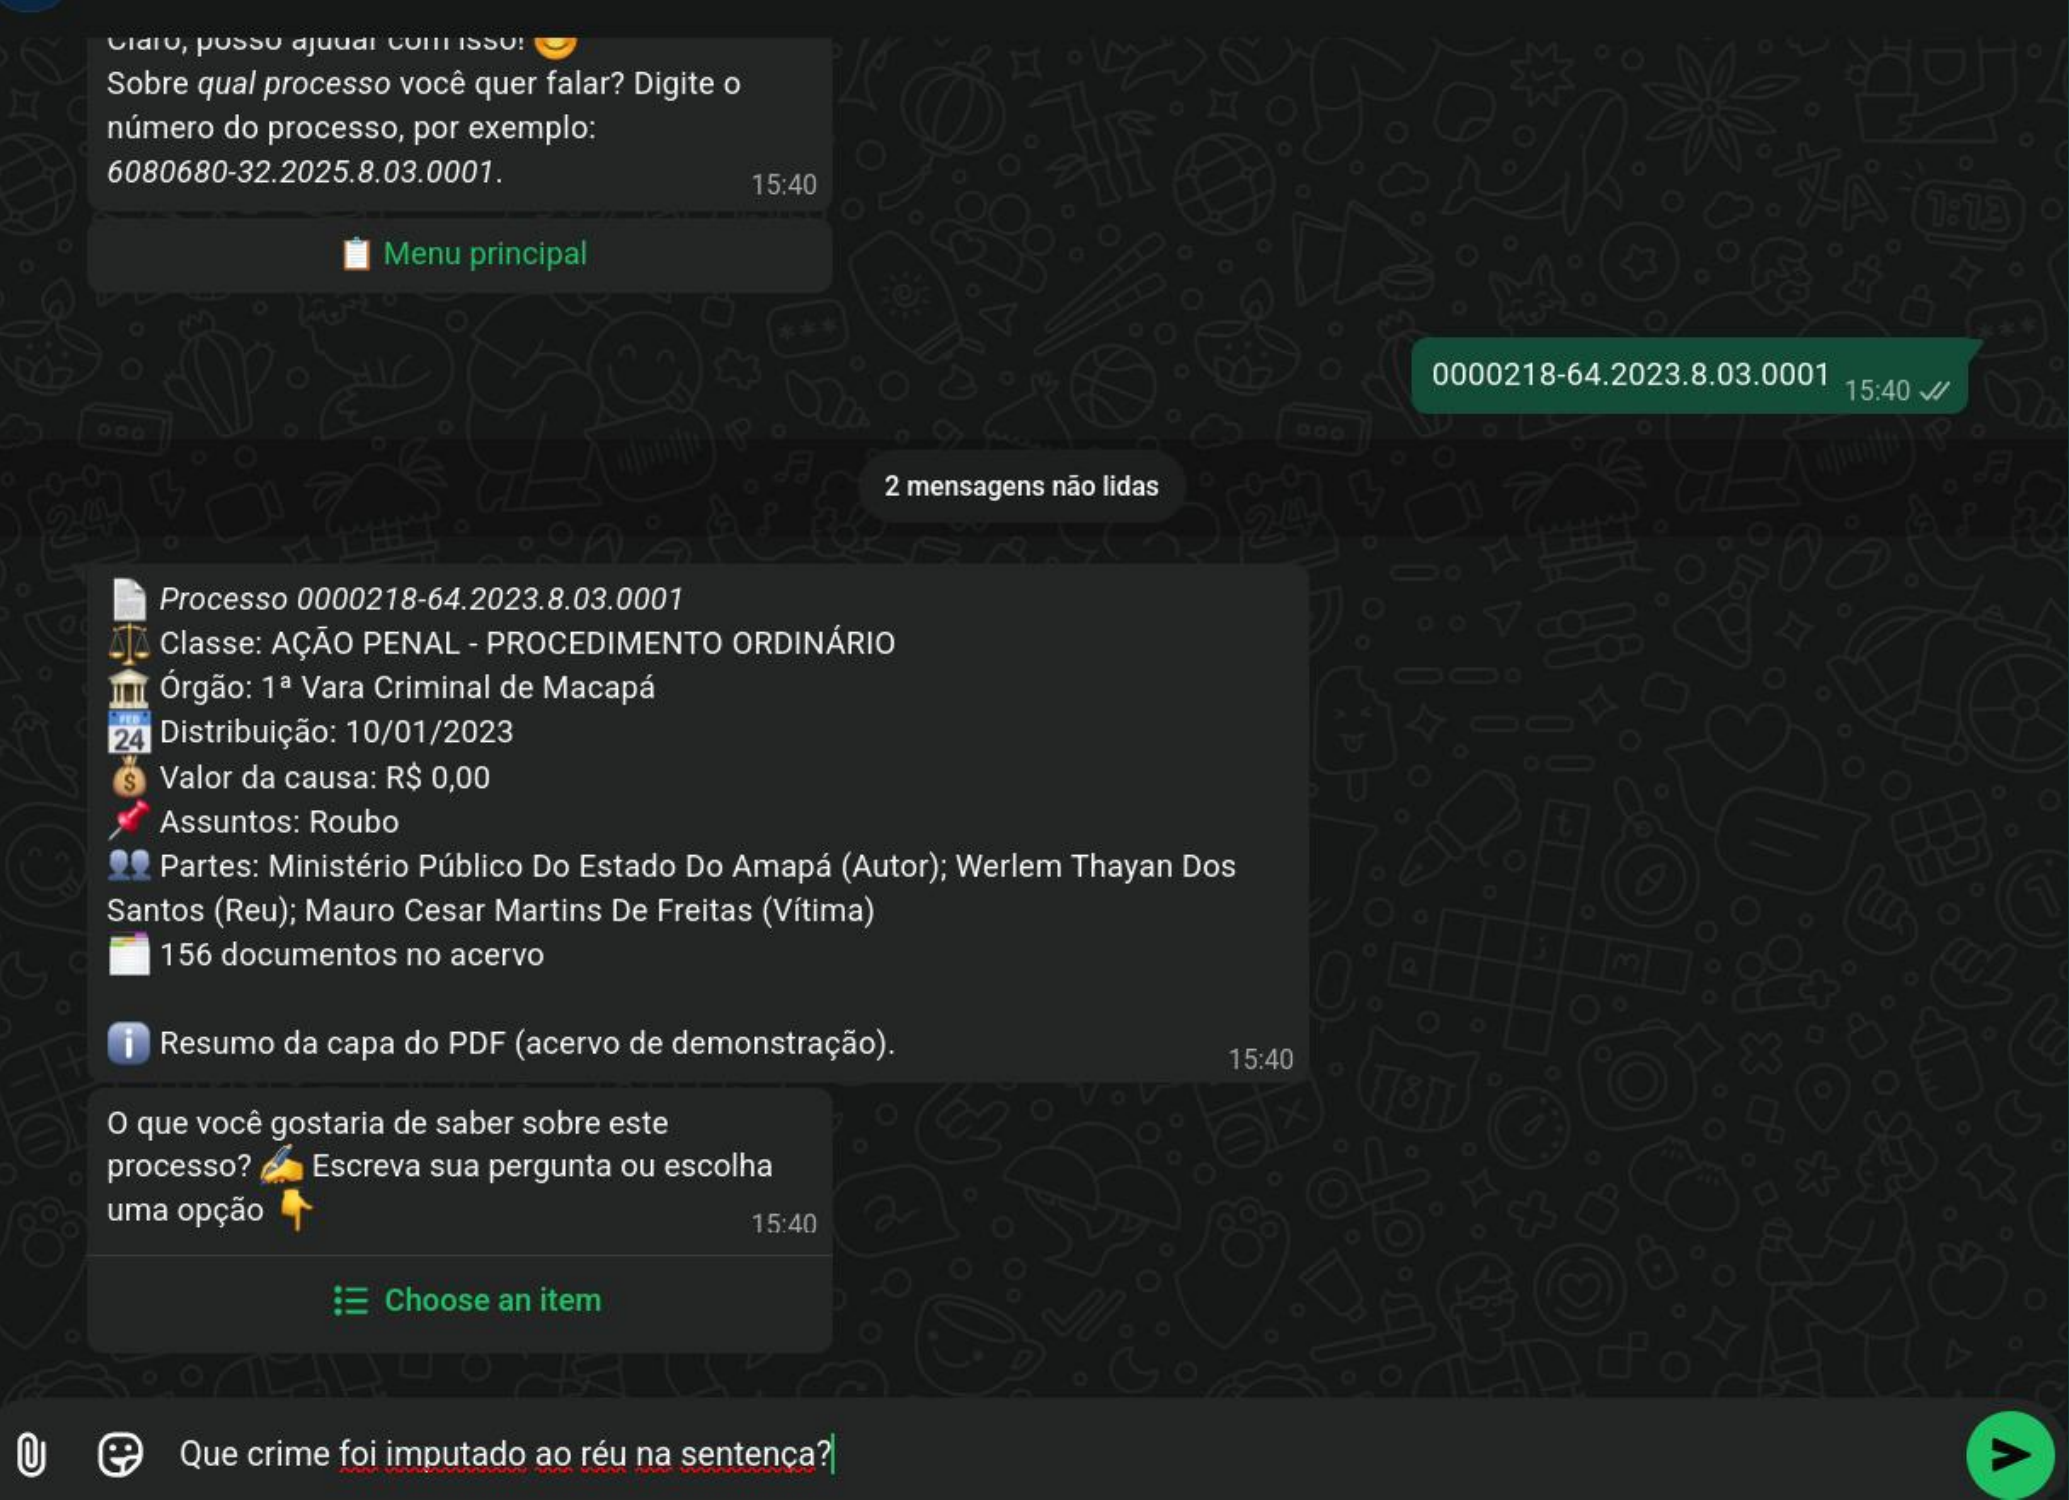
\includegraphics[width=\linewidth]{img/whatsapp_demo_processo.png}\\
      {\tiny\textcolor{cinza}{Conversa real no WhatsApp do piloto, com processo do acervo de demonstração.}}
    \column{0.42\textwidth}
      \small
      \textbf{\textcolor{petroleo}{Entregue e implantado na VM do projeto}}
      \begin{itemize}\setlength\itemsep{3pt}
        \item WhatsApp ligado ao Chatwoot, com a Julia como agente bot
        \item resumo do processo a partir da capa do PDF, e perguntas em sequência sem repetir o número
        \item menus com botões, ticket TKT e encerramento por atendente, menu ou inatividade
        \item tela de curadoria: nada coletado vai ao ar sem aprovação humana
        \item 319 testes automatizados passando
      \end{itemize}
  \end{columns}
\end{frame}

% ==========================================================================
% 15. VALIDAÇÃO INTERNA
% ==========================================================================
\begin{frame}{O que medimos até agora}
  \begin{columns}[T]
    \column{0.48\textwidth}
      \textbf{\textcolor{petroleo}{\faDatabase\ Acervo de demonstração}}\\[4pt]
      \small
      \begin{tabularx}{\linewidth}{@{}X r@{}}
        \toprule
        Processos em PDF                       & 10 \\
        Páginas lidas (362 com OCR)            & 7.893 \\
        Documentos catalogados                 & 892 \\
        Trechos indexados para busca           & 17.357 \\
        Dados pessoais no índice (CPF, RG\dots) & 0 \\
        \bottomrule
      \end{tabularx}
    \column{0.48\textwidth}
      \textbf{\textcolor{petroleo}{\faClipboardCheck\ Perguntas de teste, ponta a ponta}}\\[4pt]
      \small
      \begin{tabularx}{\linewidth}{@{}X r@{}}
        \toprule
        Respostas aprovadas                    & 40 de 42 \\
        Respostas com fonte citada             & 100\% \\
        Respostas com números conferidos       & 100\% \\
        Achar o trecho certo entre os 6 primeiros & 25 de 28 \\
        Tempo típico de resposta               & cerca de 2 s \\
        \bottomrule
      \end{tabularx}
  \end{columns}
  \vfill
  \begin{tikzpicture}
    \node[fill=areia,rounded corners=4pt,text width=13.9cm,inner sep=6pt,font=\scriptsize,text=ambar!40!black]
      {\faInfoCircle\ Leitura honesta: são testes internos com 42 perguntas sobre o acervo de demonstração (processos do TJAP cedidos para o desafio), parte delas usada para ajustar o sistema. Mostram que a engenharia funciona. O ganho no atendimento real só aparece no piloto, e é isso que propomos medir.};
  \end{tikzpicture}
\end{frame}

% ==========================================================================
% 16. EVIDÊNCIAS DE MERCADO
% ==========================================================================
\begin{frame}{O que o mercado já mostrou}
  \scriptsize
  \renewcommand{\arraystretch}{1.25}
  \begin{tabularx}{\linewidth}{@{}>{\raggedright\arraybackslash}p{3.0cm} >{\raggedright\arraybackslash}p{3.3cm} X@{}}
    \toprule
    \textbf{Fonte} & \textbf{Contexto} & \textbf{Achado} \\
    \midrule
    Brynjolfsson, Li e Raymond \cite{brynjolfsson2023} & 5.179 atendentes de suporte com assistente de IA & \textbf{+14\%} de casos resolvidos por hora, \textbf{+34\%} entre os novatos, clientes mais satisfeitos \\
    Gartner \cite{gartner2022} & previsão para centrais de atendimento & IA conversacional deve cortar \textbf{US\$ 80 bilhões} em custo de mão de obra em 2026, com bots coletando dados e passando ao humano \\
    Klarna \cite{klarna2024} & assistente de IA no atendimento, dados da própria empresa & \textbf{2/3} dos chats no primeiro mês, tempo de resolução de \textbf{11 para menos de 2 minutos} \\
    Mobile Time e Opinion Box \cite{mobiletime2020} & uso de mensageiros no Brasil & WhatsApp em \textbf{99\%} dos smartphones, \textbf{93\%} abrem o app todo dia \\
    \bottomrule
  \end{tabularx}
  \vfill
  {\small O padrão se repete: a IA resolve o volume repetitivo e o humano fica com os casos que precisam de julgamento.}
\end{frame}

% ==========================================================================
% 17. EVIDÊNCIAS CIENTÍFICAS E SETOR PÚBLICO
% ==========================================================================
\begin{frame}{O que a pesquisa e o Judiciário já mostraram}
  \scriptsize
  \renewcommand{\arraystretch}{1.25}
  \begin{tabularx}{\linewidth}{@{}>{\raggedright\arraybackslash}p{3.0cm} >{\raggedright\arraybackslash}p{3.3cm} X@{}}
    \toprule
    \textbf{Fonte} & \textbf{Contexto} & \textbf{Achado} \\
    \midrule
    Lewis et al.\ \cite{lewis2020} & NeurIPS 2020 & buscar documentos antes de gerar produz respostas mais específicas e factuais \\
    Shuster et al.\ \cite{shuster2021} & EMNLP 2021 & a recuperação reduz respostas alucinadas em \textbf{mais de 60\%} \\
    Magesh et al.\ \cite{magesh2025} & ferramentas jurídicas comerciais & mesmo com RAG, erram entre \textbf{17\% e 33\%}. Verificar a resposta é obrigatório \\
    TJCE \cite{tjce} & robô no WhatsApp Business da Secretaria Judiciária & \textbf{285 pessoas} atendidas na primeira semana, e em outra unidade \textbf{3 colaboradores} liberados para outros canais \\
    CNJ \cite{cnj372,cnj615} & Res.\ 372/2021 e 615/2025 & Balcão Virtual obrigatório com ferramenta livre, e IA com supervisão humana e transparência \\
    \bottomrule
  \end{tabularx}
  \vfill
  {\small A EscutAI junta as duas lições: atendimento automatizado no canal que o cidadão já usa, com verificação e um humano sempre a um toque.}
\end{frame}

% ==========================================================================
% 18. GOVERNANÇA E CONFORMIDADE
% ==========================================================================
\begin{frame}{Pronta para as regras do Judiciário}
  \centering
  \begin{tikzpicture}[x=1cm,y=1cm,
      card/.style={caixa,fill=nevoa,text width=3.9cm,minimum height=3.6cm,font=\scriptsize,align=left,anchor=north}]
    \node[card] at (0,0) {{\Large\textcolor{verde}{\faUserShield}}\\[3pt]\textbf{\small Supervisão humana}\\[3pt]
      A Julia nunca decide nada. Ela informa o que está nos autos e passa ao servidor tudo o que pede análise, como pede a Res.\ CNJ 615/2025.};
    \node[card] at (4.6,0) {{\Large\textcolor{verde}{\faLock}}\\[3pt]\textbf{\small LGPD}\\[3pt]
      CPF, RG, telefone e e-mail são mascarados antes da indexação. Processos em segredo de justiça ficam fora. Chaves e dados ficam no servidor do Tribunal.};
    \node[card] at (9.2,0) {{\Large\textcolor{verde}{\faClipboardList}}\\[3pt]\textbf{\small Rastreabilidade}\\[3pt]
      Cada resposta guarda as fontes usadas. Cada atendimento tem ticket, horário de abertura e de encerramento, e trilha de auditoria.};
  \end{tikzpicture}
  \vfill
  {\small Software livre (Chatwoot, licença MIT) instalado em infraestrutura própria. O Tribunal não fica preso a um fornecedor.}
\end{frame}

% ==========================================================================
% 18b. PROPOSTA PRELIMINAR
% ==========================================================================
\begin{frame}{Proposta preliminar para o TJPA}
  \begin{columns}[T]
    \column{0.31\textwidth}
      \begin{tikzpicture}
        \node[caixa,fill=nevoa,text width=4.1cm,minimum height=3.2cm,align=left,font=\scriptsize,anchor=north] {%
          {\small\bfseries\textcolor{petroleo}{\faBullseye\ Escopo do piloto}}\\[4pt]
          \textbullet\ 1 ou 2 unidades judiciárias escolhidas pelo TJPA\\[2pt]
          \textbullet\ WhatsApp oficial do Tribunal ligado ao Chatwoot\\[2pt]
          \textbullet\ Julia respondendo sobre processos, serviços do Tribunal e orientação jurídica básica\\[2pt]
          \textbullet\ transferência para servidores da própria unidade};
      \end{tikzpicture}
    \column{0.31\textwidth}
      \begin{tikzpicture}
        \node[caixa,fill=nevoa,text width=4.1cm,minimum height=3.2cm,align=left,font=\scriptsize,anchor=north] {%
          {\small\bfseries\textcolor{petroleo}{\faBoxOpen\ O que entregamos}}\\[4pt]
          \textbullet\ instalação em servidor do TJPA\\[2pt]
          \textbullet\ base de conhecimento inicial, curada com a unidade\\[2pt]
          \textbullet\ painel de curadoria, tickets e indicadores\\[2pt]
          \textbullet\ capacitação dos servidores\\[2pt]
          \textbullet\ relatório final com os indicadores medidos};
      \end{tikzpicture}
    \column{0.31\textwidth}
      \begin{tikzpicture}
        \node[caixa,fill=areia,text width=4.1cm,minimum height=3.2cm,align=left,font=\scriptsize,anchor=north,text=ambar!35!black] {%
          {\small\bfseries\faHandshake\ O que precisamos do TJPA}\\[4pt]
          \textbullet\ número de WhatsApp Business oficial\\[2pt]
          \textbullet\ acesso autorizado aos dados processuais (API ou exportação)\\[2pt]
          \textbullet\ um ou dois servidores curadores por unidade\\[2pt]
          \textbullet\ aval da área de proteção de dados e do comitê de IA};
      \end{tikzpicture}
  \end{columns}
  \vspace{0.1cm}

  \scriptsize
  \begin{tabularx}{\linewidth}{@{}l l X@{}}
    \toprule
    \textbf{Semanas} & \textbf{Etapa} & \textbf{Marco de saída} \\
    \midrule
    1 a 2   & Preparação          & número oficial ativo, sistema instalado, base inicial aprovada \\
    3 a 4   & Operação assistida  & servidores revisam as respostas da Julia antes de liberar o atendimento pleno \\
    5 a 10  & Operação e medição  & indicadores coletados toda semana e comparados com a linha de base \\
    11 a 12 & Avaliação           & relatório de resultados e decisão conjunta sobre a expansão \\
    \bottomrule
  \end{tabularx}\\[2pt]
  {\tiny\textcolor{cinza}{Cronograma preliminar de 12 semanas, a ajustar com o TJPA.}}
\end{frame}

% ==========================================================================
% 19. ROADMAP DO PILOTO
% ==========================================================================
\begin{frame}{Do piloto ao estado inteiro}
  \centering
  \begin{tikzpicture}[x=1cm,y=1cm,
      fase/.style={caixa,fill=nevoa,text width=3.95cm,font=\scriptsize,align=left,anchor=north}]
    \draw[line width=3pt,seta,-{Triangle[width=9pt,length=7pt]}] (-0.6,0) -- (13.6,0);
    \node[marco=verde] (m1) at (1.4,0) {1};
    \node[marco=petroleo] (m2) at (6.3,0) {2};
    \node[marco=ambar] (m3) at (11.2,0) {3};
    \node[font=\small\bfseries,above=3pt of m1] {Piloto assistido};
    \node[font=\small\bfseries,above=3pt of m2] {Integração};
    \node[font=\small\bfseries,above=3pt of m3] {Expansão};
    \node[fase] at (1.4,-0.5) {\textbf{1 ou 2 unidades}\\[2pt]
      \textbullet\ WhatsApp oficial + Chatwoot + Julia\\
      \textbullet\ base curada pela própria unidade\\
      \textbullet\ revisão humana de amostra das respostas\\
      \textbullet\ linha de base dos indicadores};
    \node[fase] at (6.3,-0.5) {\textbf{API processual e Balcão Virtual}\\[2pt]
      \textbullet\ andamento direto da API oficial do PJe\\
      \textbullet\ e-mail na mesma caixa do WhatsApp\\
      \textbullet\ painel com filas e tempos por unidade};
    \node[fase] at (11.2,-0.5) {\textbf{Até as 299 unidades}\\[2pt]
      \textbullet\ entrada por ondas, por comarca\\
      \textbullet\ times e etiquetas por unidade\\
      \textbullet\ treinamento curto dos servidores\\
      \textbullet\ relatório público de resultados};
  \end{tikzpicture}
  \vfill
  {\tiny\textcolor{cinza}{Sequência proposta pela equipe. Prazos de cada fase a definir com o TJPA conforme a disponibilidade da API processual e a homologação do número oficial.}}
\end{frame}

% ==========================================================================
% 20. RESULTADOS ESPERADOS E COMO MEDIR
% ==========================================================================
\begin{frame}{Resultados esperados e métricas}
  \footnotesize
  \renewcommand{\arraystretch}{1.2}
  \begin{tabularx}{\linewidth}{@{}>{\raggedright\arraybackslash}p{4.3cm} X >{\raggedright\arraybackslash}p{2.6cm}@{}}
    \toprule
    \textbf{Resultado esperado} & \textbf{Indicador no piloto} & \textbf{Fonte do dado} \\
    \midrule
    Menos atendimentos que exigem humano & \% de conversas encerradas sem transferência & Chatwoot \\
    Mais resolução no primeiro contato & \% de tickets sem reabertura em 7 dias & tickets TKT \\
    Encaminhamento correto & \% de transferências que chegam ao time certo & etiquetas e times \\
    Resposta mais rápida & tempo até a primeira resposta e até o encerramento & Chatwoot \\
    Menos deslocamento presencial & resposta à pergunta ``isso evitou uma ida ao fórum?'' & pesquisa no encerramento \\
    Atendimento rastreável & \% de conversas com ticket, fonte e horário & trilha de auditoria \\
    \bottomrule
  \end{tabularx}
  \vfill
  {\small Os percentuais entram aqui depois das primeiras semanas de piloto, comparados com a linha de base da unidade. Não vamos prometer número antes de medir.}
\end{frame}

% ==========================================================================
% 21. DIFERENCIAIS
% ==========================================================================
\begin{frame}{Por que a EscutAI}
  \begin{columns}[c]
    \column{0.6\textwidth}
      \small
      \begin{itemize}\setlength\itemsep{6pt}
        \item Atende jurisdicionados (partes e testemunhas), advogados e servidores das \textbf{299 unidades}.
        \item Torna o WhatsApp um canal \textbf{oficial e centralizado}, com linguagem simples para o público leigo.
        \item Usa o que o Tribunal já tem: canal de mensagens, servidores próprios e APIs. Continua depois do hackathon.
        \item Responde com fonte e admite quando não sabe. O servidor recebe só o que precisa dele.
        \item Já está funcionando. O piloto começa pela configuração, não pelo desenvolvimento.
      \end{itemize}
    \column{0.37\textwidth}\centering
      \begin{tikzpicture}
        \clip[rounded corners=8pt] (0,0) rectangle (4.5,5.2);
        \node[anchor=south west,inner sep=0] at (0,0) {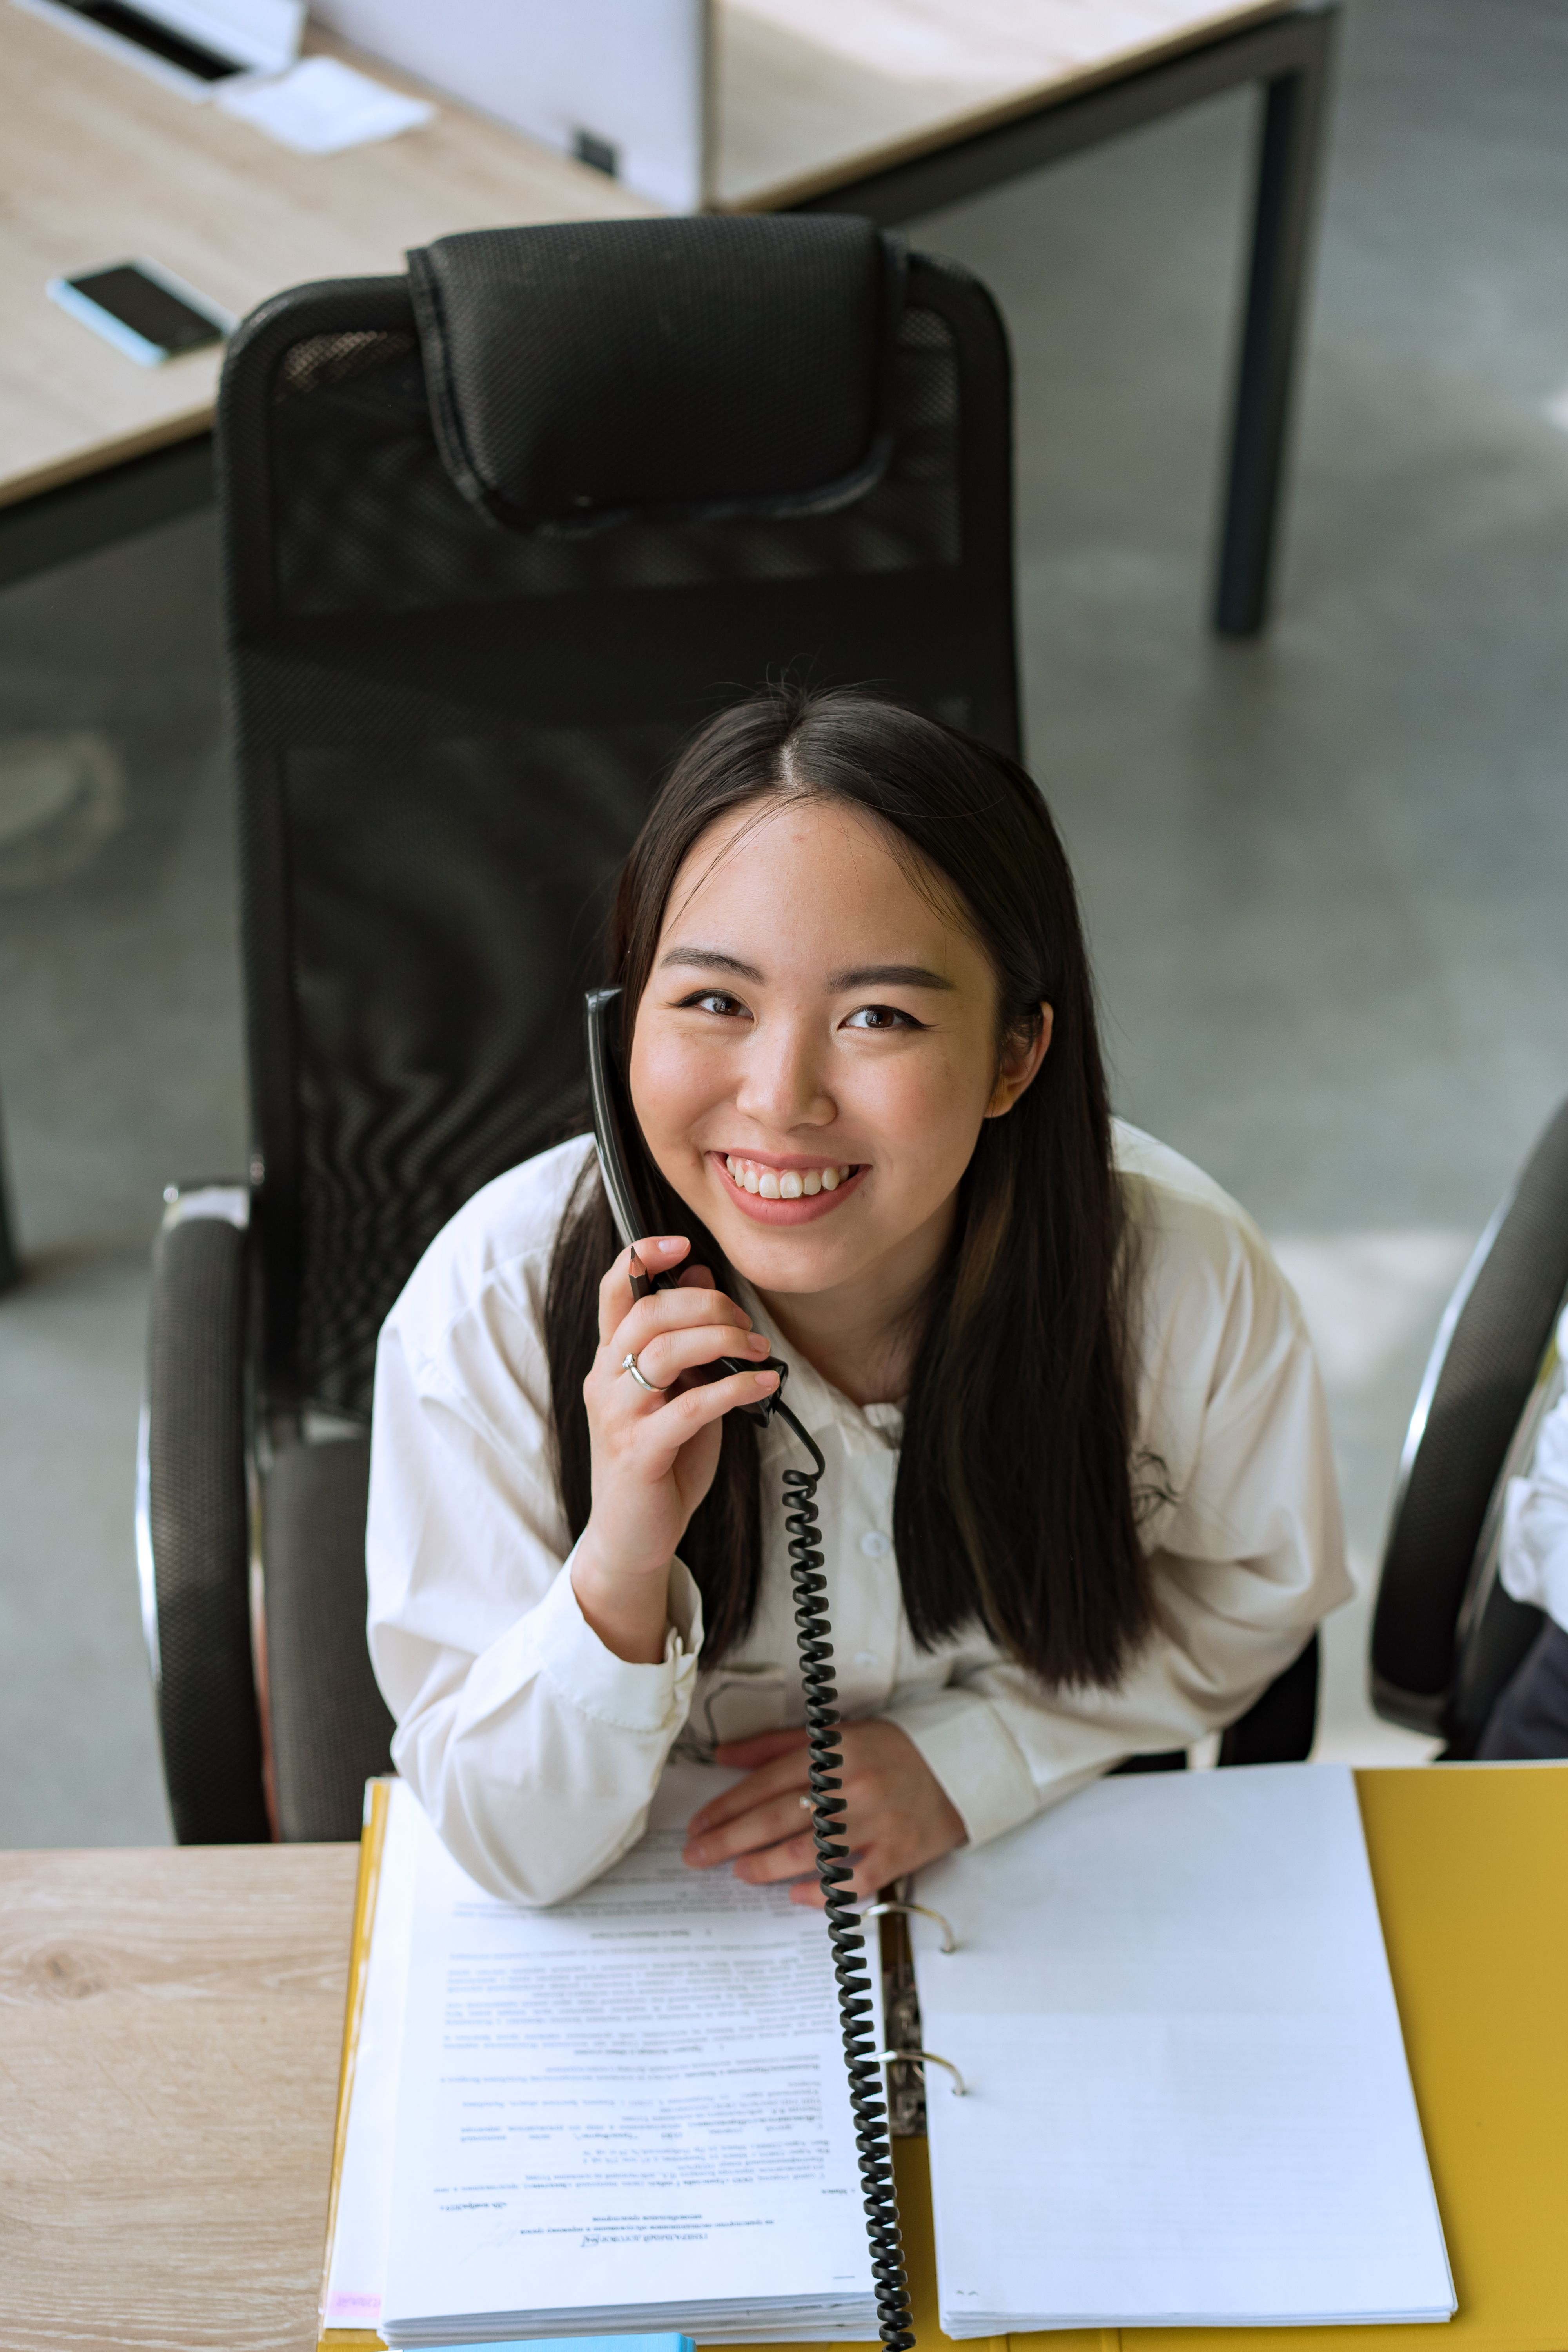
\includegraphics[width=4.5cm,height=5.2cm,keepaspectratio=false]{img/servidora_atendimento.jpg}};
      \end{tikzpicture}\\[3pt]
      {\tiny\textcolor{cinza}{Foto: Mikhail Nilov, Pexels}}
  \end{columns}
\end{frame}

% ==========================================================================
% 22. CITAÇÃO
% ==========================================================================
{\fundoescuro
\begin{frame}[plain]
  \begin{columns}[c]
    \column{0.72\textwidth}
      \textcolor{ambar}{\Huge\faCircle}\\[0.5cm]
      {\fontsize{24}{30}\selectfont\bfseries\itshape ``Cada dúvida resolvida no primeiro contato é \textcolor{ambar}{um cidadão atendido} e \textcolor{menta}{um servidor liberado}.''}\\[0.5cm]
      {\small\textcolor{menta!60!white}{Equipe EscutAI}}
    \column{0.26\textwidth}\centering
      \vspace{2.5cm}
      
\includegraphics[width=\linewidth]{img/julia_encaminhando.png}
  \end{columns}
\end{frame}
}

% ==========================================================================
% 23. OBRIGADO
% ==========================================================================
{\fundoescuro
\begin{frame}[plain]
  \centering
  
\includegraphics[height=2.3cm]{img/logo_escutai_branco.png}\\[0.2cm]
  {\fontsize{26}{28}\selectfont\bfseries Escut\textcolor{menta}{AI}}\\[0.5cm]
  {\fontsize{30}{32}\selectfont\bfseries Obrigado!}\\[0.5cm]
  {\small\textcolor{white!85}{\faUser\ Carlos Portela \quad\faEnvelope\ csp@ufpa.br \quad\faPhone\ (91) 98065-6772}}\\[0.9cm]
  {\small\textcolor{menta}{A Justiça que escuta você.}}
\end{frame}
}

% ==========================================================================
% 24. REFERÊNCIAS
% ==========================================================================
\begin{frame}{Referências}
  \tiny
  \begin{thebibliography}{99}
    \setbeamertemplate{bibliography item}[text]
    \bibitem{brynjolfsson2023} E. Brynjolfsson, D. Li e L. Raymond. \emph{Generative AI at Work}. NBER Working Paper 31161, 2023. \url{https://www.nber.org/papers/w31161}
    \bibitem{cnj2025} Conselho Nacional de Justiça. \emph{Justiça em Números 2025}: sumário executivo. Brasília: CNJ, 2025. \url{https://www.cnj.jus.br/wp-content/uploads/2025/10/sumario-executivo-2025.pdf}
    \bibitem{cnj372} Conselho Nacional de Justiça. Resolução nº 372, de 12 de fevereiro de 2021 (Balcão Virtual), alterada pela Resolução nº 473/2022. \url{https://atos.cnj.jus.br/atos/detalhar/3742}
    \bibitem{cnj615} Conselho Nacional de Justiça. Resolução nº 615, de 11 de março de 2025. Diretrizes para desenvolvimento, uso e governança de IA no Poder Judiciário.
    \bibitem{gartner2022} Gartner. \emph{Gartner Predicts Conversational AI Will Reduce Contact Center Agent Labor Costs by \$80 Billion in 2026}. Comunicado de imprensa, 31 ago. 2022. Repercutido em \url{https://www.cxtoday.com/workforce-engagement-management/gartner-bots-cut-agent-labor-costs-80bn/}
    \bibitem{klarna2024} Klarna. \emph{Klarna AI assistant handles two-thirds of customer service chats in its first month}. Comunicado de imprensa, fev. 2024 (dados informados pela empresa). Repercutido em \url{https://www.cxtoday.com/contact-center/klarna-claims-its-new-ai-assistant-does-the-work-of-700-full-time-agents/}
    \bibitem{lewis2020} P. Lewis et al. Retrieval-Augmented Generation for Knowledge-Intensive NLP Tasks. \emph{NeurIPS}, v. 33, p. 9459--9474, 2020. arXiv:2005.11401.
    \bibitem{magesh2025} V. Magesh, F. Surani, M. Dahl, M. Suzgun, C. D. Manning e D. E. Ho. Hallucination-Free? Assessing the Reliability of Leading AI Legal Research Tools. \emph{Journal of Empirical Legal Studies}, v. 22, p. 216--242, 2025. DOI 10.1111/jels.12413.
    \bibitem{mobiletime2020} Mobile Time e Opinion Box. \emph{Panorama Mensageria no Brasil}, fev. 2020. Repercutido em \url{https://www.hardware.com.br/noticias/2020-02/whatsapp-esta-presente-em-99-dos-celulares-no-brasil.html}
    \bibitem{shuster2021} K. Shuster, S. Poff, M. Chen, D. Kiela e J. Weston. Retrieval Augmentation Reduces Hallucination in Conversation. \emph{Findings of EMNLP 2021}, p. 3784--3803. DOI 10.18653/v1/2021.findings-emnlp.320.
    \bibitem{tjce} Tribunal de Justiça do Ceará. \emph{TJCE implanta robô na Secretaria Judiciária de Fortaleza}. Notícia institucional, s.d. \url{https://www.tjce.jus.br/noticias/tjce-implanta-robo-na-secretaria-judiciaria-de-fortaleza-e-aumenta-em-mais-de-2-600-o-numero-de-movimentacoes-processuais/}
  \end{thebibliography}
\end{frame}

\end{document}
